% Gemini theme
% https://github.com/anishathalye/gemini

\documentclass[final]{beamer}

% ====================
% Packages
% ====================

\usepackage[T1]{fontenc}
\usepackage{lmodern}
\usepackage[size=custom,width=120,height=72,scale=1.0]{beamerposter}
\usetheme{gemini}
\usecolortheme{gemini}
\usepackage{graphicx}
\usepackage{booktabs}
\usepackage{tikz}
\usepackage{pgfplots}

%%%%% NEW MATH DEFINITIONS %%%%%
\usepackage{amsmath,amsfonts,bm}

% Random variables
\def\reta{{\textnormal{$\eta$}}}
\def\ra{{\textnormal{a}}}
\def\rb{{\textnormal{b}}}
\def\rc{{\textnormal{c}}}
\def\rd{{\textnormal{d}}}
\def\re{{\textnormal{e}}}
\def\rf{{\textnormal{f}}}
\def\rg{{\textnormal{g}}}
\def\rh{{\textnormal{h}}}
\def\ri{{\textnormal{i}}}
\def\rj{{\textnormal{j}}}
\def\rk{{\textnormal{k}}}
\def\rl{{\textnormal{l}}}
% rm is already a command, just don't name any random variables m
\def\rn{{\textnormal{n}}}
\def\ro{{\textnormal{o}}}
\def\rp{{\textnormal{p}}}
\def\rq{{\textnormal{q}}}
\def\rr{{\textnormal{r}}}
\def\rs{{\textnormal{s}}}
\def\rt{{\textnormal{t}}}
\def\ru{{\textnormal{u}}}
\def\rv{{\textnormal{v}}}
\def\rw{{\textnormal{w}}}
\def\rx{{\textnormal{x}}}
\def\ry{{\textnormal{y}}}
\def\rz{{\textnormal{z}}}

% Random vectors
\def\rvepsilon{{\mathbf{\epsilon}}}
\def\rvtheta{{\mathbf{\theta}}}
\def\rva{{\mathbf{a}}}
\def\rvb{{\mathbf{b}}}
\def\rvc{{\mathbf{c}}}
\def\rvd{{\mathbf{d}}}
\def\rve{{\mathbf{e}}}
\def\rvf{{\mathbf{f}}}
\def\rvg{{\mathbf{g}}}
\def\rvh{{\mathbf{h}}}
\def\rvu{{\mathbf{i}}}
\def\rvj{{\mathbf{j}}}
\def\rvk{{\mathbf{k}}}
\def\rvl{{\mathbf{l}}}
\def\rvm{{\mathbf{m}}}
\def\rvn{{\mathbf{n}}}
\def\rvo{{\mathbf{o}}}
\def\rvp{{\mathbf{p}}}
\def\rvq{{\mathbf{q}}}
\def\rvr{{\mathbf{r}}}
\def\rvs{{\mathbf{s}}}
\def\rvt{{\mathbf{t}}}
\def\rvu{{\mathbf{u}}}
\def\rvv{{\mathbf{v}}}
\def\rvw{{\mathbf{w}}}
\def\rvx{{\mathbf{x}}}
\def\rvy{{\mathbf{y}}}
\def\rvz{{\mathbf{z}}}

% Elements of random vectors
\def\erva{{\textnormal{a}}}
\def\ervb{{\textnormal{b}}}
\def\ervc{{\textnormal{c}}}
\def\ervd{{\textnormal{d}}}
\def\erve{{\textnormal{e}}}
\def\ervf{{\textnormal{f}}}
\def\ervg{{\textnormal{g}}}
\def\ervh{{\textnormal{h}}}
\def\ervi{{\textnormal{i}}}
\def\ervj{{\textnormal{j}}}
\def\ervk{{\textnormal{k}}}
\def\ervl{{\textnormal{l}}}
\def\ervm{{\textnormal{m}}}
\def\ervn{{\textnormal{n}}}
\def\ervo{{\textnormal{o}}}
\def\ervp{{\textnormal{p}}}
\def\ervq{{\textnormal{q}}}
\def\ervr{{\textnormal{r}}}
\def\ervs{{\textnormal{s}}}
\def\ervt{{\textnormal{t}}}
\def\ervu{{\textnormal{u}}}
\def\ervv{{\textnormal{v}}}
\def\ervw{{\textnormal{w}}}
\def\ervx{{\textnormal{x}}}
\def\ervy{{\textnormal{y}}}
\def\ervz{{\textnormal{z}}}

% Random matrices
\def\rmA{{\mathbf{A}}}
\def\rmB{{\mathbf{B}}}
\def\rmC{{\mathbf{C}}}
\def\rmD{{\mathbf{D}}}
\def\rmE{{\mathbf{E}}}
\def\rmF{{\mathbf{F}}}
\def\rmG{{\mathbf{G}}}
\def\rmH{{\mathbf{H}}}
\def\rmI{{\mathbf{I}}}
\def\rmJ{{\mathbf{J}}}
\def\rmK{{\mathbf{K}}}
\def\rmL{{\mathbf{L}}}
\def\rmM{{\mathbf{M}}}
\def\rmN{{\mathbf{N}}}
\def\rmO{{\mathbf{O}}}
\def\rmP{{\mathbf{P}}}
\def\rmQ{{\mathbf{Q}}}
\def\rmR{{\mathbf{R}}}
\def\rmS{{\mathbf{S}}}
\def\rmT{{\mathbf{T}}}
\def\rmU{{\mathbf{U}}}
\def\rmV{{\mathbf{V}}}
\def\rmW{{\mathbf{W}}}
\def\rmX{{\mathbf{X}}}
\def\rmY{{\mathbf{Y}}}
\def\rmZ{{\mathbf{Z}}}

% Elements of random matrices
\def\ermA{{\textnormal{A}}}
\def\ermB{{\textnormal{B}}}
\def\ermC{{\textnormal{C}}}
\def\ermD{{\textnormal{D}}}
\def\ermE{{\textnormal{E}}}
\def\ermF{{\textnormal{F}}}
\def\ermG{{\textnormal{G}}}
\def\ermH{{\textnormal{H}}}
\def\ermI{{\textnormal{I}}}
\def\ermJ{{\textnormal{J}}}
\def\ermK{{\textnormal{K}}}
\def\ermL{{\textnormal{L}}}
\def\ermM{{\textnormal{M}}}
\def\ermN{{\textnormal{N}}}
\def\ermO{{\textnormal{O}}}
\def\ermP{{\textnormal{P}}}
\def\ermQ{{\textnormal{Q}}}
\def\ermR{{\textnormal{R}}}
\def\ermS{{\textnormal{S}}}
\def\ermT{{\textnormal{T}}}
\def\ermU{{\textnormal{U}}}
\def\ermV{{\textnormal{V}}}
\def\ermW{{\textnormal{W}}}
\def\ermX{{\textnormal{X}}}
\def\ermY{{\textnormal{Y}}}
\def\ermZ{{\textnormal{Z}}}

% Vectors
\def\vzero{{\bm{0}}}
\def\vone{{\bm{1}}}
\def\vmu{{\bm{\mu}}}
\def\vtheta{{\bm{\theta}}}
\def\va{{\bm{a}}}
\def\vb{{\bm{b}}}
\def\vc{{\bm{c}}}
\def\vd{{\bm{d}}}
\def\ve{{\bm{e}}}
\def\vf{{\bm{f}}}
\def\vg{{\bm{g}}}
\def\vh{{\bm{h}}}
\def\vi{{\bm{i}}}
\def\vj{{\bm{j}}}
\def\vk{{\bm{k}}}
\def\vl{{\bm{l}}}
\def\vm{{\bm{m}}}
\def\vn{{\bm{n}}}
\def\vo{{\bm{o}}}
\def\vp{{\bm{p}}}
\def\vq{{\bm{q}}}
\def\vr{{\bm{r}}}
\def\vs{{\bm{s}}}
\def\vt{{\bm{t}}}
\def\vu{{\bm{u}}}
\def\vv{{\bm{v}}}
\def\vw{{\bm{w}}}
\def\vx{{\bm{x}}}
\def\vy{{\bm{y}}}
\def\vz{{\bm{z}}}

% Elements of vectors
\def\evalpha{{\alpha}}
\def\evbeta{{\beta}}
\def\evepsilon{{\epsilon}}
\def\evlambda{{\lambda}}
\def\evomega{{\omega}}
\def\evmu{{\mu}}
\def\evpsi{{\psi}}
\def\evsigma{{\sigma}}
\def\evtheta{{\theta}}
\def\eva{{a}}
\def\evb{{b}}
\def\evc{{c}}
\def\evd{{d}}
\def\eve{{e}}
\def\evf{{f}}
\def\evg{{g}}
\def\evh{{h}}
\def\evi{{i}}
\def\evj{{j}}
\def\evk{{k}}
\def\evl{{l}}
\def\evm{{m}}
\def\evn{{n}}
\def\evo{{o}}
\def\evp{{p}}
\def\evq{{q}}
\def\evr{{r}}
\def\evs{{s}}
\def\evt{{t}}
\def\evu{{u}}
\def\evv{{v}}
\def\evw{{w}}
\def\evx{{x}}
\def\evy{{y}}
\def\evz{{z}}

% Matrix
\def\mA{{\bm{A}}}
\def\mB{{\bm{B}}}
\def\mC{{\bm{C}}}
\def\mD{{\bm{D}}}
\def\mE{{\bm{E}}}
\def\mF{{\bm{F}}}
\def\mG{{\bm{G}}}
\def\mH{{\bm{H}}}
\def\mI{{\bm{I}}}
\def\mJ{{\bm{J}}}
\def\mK{{\bm{K}}}
\def\mL{{\bm{L}}}
\def\mM{{\bm{M}}}
\def\mN{{\bm{N}}}
\def\mO{{\bm{O}}}
\def\mP{{\bm{P}}}
\def\mQ{{\bm{Q}}}
\def\mR{{\bm{R}}}
\def\mS{{\bm{S}}}
\def\mT{{\bm{T}}}
\def\mU{{\bm{U}}}
\def\mV{{\bm{V}}}
\def\mW{{\bm{W}}}
\def\mX{{\bm{X}}}
\def\mY{{\bm{Y}}}
\def\mZ{{\bm{Z}}}
\def\mBeta{{\bm{\beta}}}
\def\mPhi{{\bm{\Phi}}}
\def\mLambda{{\bm{\Lambda}}}
\def\mSigma{{\bm{\Sigma}}}

% Tensor
\DeclareMathAlphabet{\mathsfit}{\encodingdefault}{\sfdefault}{m}{sl}
\SetMathAlphabet{\mathsfit}{bold}{\encodingdefault}{\sfdefault}{bx}{n}
\newcommand{\tens}[1]{\bm{\mathsfit{#1}}}
\def\tA{{\tens{A}}}
\def\tB{{\tens{B}}}
\def\tC{{\tens{C}}}
\def\tD{{\tens{D}}}
\def\tE{{\tens{E}}}
\def\tF{{\tens{F}}}
\def\tG{{\tens{G}}}
\def\tH{{\tens{H}}}
\def\tI{{\tens{I}}}
\def\tJ{{\tens{J}}}
\def\tK{{\tens{K}}}
\def\tL{{\tens{L}}}
\def\tM{{\tens{M}}}
\def\tN{{\tens{N}}}
\def\tO{{\tens{O}}}
\def\tP{{\tens{P}}}
\def\tQ{{\tens{Q}}}
\def\tR{{\tens{R}}}
\def\tS{{\tens{S}}}
\def\tT{{\tens{T}}}
\def\tU{{\tens{U}}}
\def\tV{{\tens{V}}}
\def\tW{{\tens{W}}}
\def\tX{{\tens{X}}}
\def\tY{{\tens{Y}}}
\def\tZ{{\tens{Z}}}


% Graph
\def\gA{{\mathcal{A}}}
\def\gB{{\mathcal{B}}}
\def\gC{{\mathcal{C}}}
\def\gD{{\mathcal{D}}}
\def\gE{{\mathcal{E}}}
\def\gF{{\mathcal{F}}}
\def\gG{{\mathcal{G}}}
\def\gH{{\mathcal{H}}}
\def\gI{{\mathcal{I}}}
\def\gJ{{\mathcal{J}}}
\def\gK{{\mathcal{K}}}
\def\gL{{\mathcal{L}}}
\def\gM{{\mathcal{M}}}
\def\gN{{\mathcal{N}}}
\def\gO{{\mathcal{O}}}
\def\gP{{\mathcal{P}}}
\def\gQ{{\mathcal{Q}}}
\def\gR{{\mathcal{R}}}
\def\gS{{\mathcal{S}}}
\def\gT{{\mathcal{T}}}
\def\gU{{\mathcal{U}}}
\def\gV{{\mathcal{V}}}
\def\gW{{\mathcal{W}}}
\def\gX{{\mathcal{X}}}
\def\gY{{\mathcal{Y}}}
\def\gZ{{\mathcal{Z}}}

% Sets
\def\sA{{\mathbb{A}}}
\def\sB{{\mathbb{B}}}
\def\sC{{\mathbb{C}}}
\def\sD{{\mathbb{D}}}
% Don't use a set called E, because this would be the same as our symbol
% for expectation.
\def\sF{{\mathbb{F}}}
\def\sG{{\mathbb{G}}}
\def\sH{{\mathbb{H}}}
\def\sI{{\mathbb{I}}}
\def\sJ{{\mathbb{J}}}
\def\sK{{\mathbb{K}}}
\def\sL{{\mathbb{L}}}
\def\sM{{\mathbb{M}}}
\def\sN{{\mathbb{N}}}
\def\sO{{\mathbb{O}}}
\def\sP{{\mathbb{P}}}
\def\sQ{{\mathbb{Q}}}
\def\sR{{\mathbb{R}}}
\def\sS{{\mathbb{S}}}
\def\sT{{\mathbb{T}}}
\def\sU{{\mathbb{U}}}
\def\sV{{\mathbb{V}}}
\def\sW{{\mathbb{W}}}
\def\sX{{\mathbb{X}}}
\def\sY{{\mathbb{Y}}}
\def\sZ{{\mathbb{Z}}}

% Entries of a matrix
\def\emLambda{{\Lambda}}
\def\emA{{A}}
\def\emB{{B}}
\def\emC{{C}}
\def\emD{{D}}
\def\emE{{E}}
\def\emF{{F}}
\def\emG{{G}}
\def\emH{{H}}
\def\emI{{I}}
\def\emJ{{J}}
\def\emK{{K}}
\def\emL{{L}}
\def\emM{{M}}
\def\emN{{N}}
\def\emO{{O}}
\def\emP{{P}}
\def\emQ{{Q}}
\def\emR{{R}}
\def\emS{{S}}
\def\emT{{T}}
\def\emU{{U}}
\def\emV{{V}}
\def\emW{{W}}
\def\emX{{X}}
\def\emY{{Y}}
\def\emZ{{Z}}
\def\emSigma{{\Sigma}}

% entries of a tensor
% Same font as tensor, without \bm wrapper
\newcommand{\etens}[1]{\mathsfit{#1}}
\def\etLambda{{\etens{\Lambda}}}
\def\etA{{\etens{A}}}
\def\etB{{\etens{B}}}
\def\etC{{\etens{C}}}
\def\etD{{\etens{D}}}
\def\etE{{\etens{E}}}
\def\etF{{\etens{F}}}
\def\etG{{\etens{G}}}
\def\etH{{\etens{H}}}
\def\etI{{\etens{I}}}
\def\etJ{{\etens{J}}}
\def\etK{{\etens{K}}}
\def\etL{{\etens{L}}}
\def\etM{{\etens{M}}}
\def\etN{{\etens{N}}}
\def\etO{{\etens{O}}}
\def\etP{{\etens{P}}}
\def\etQ{{\etens{Q}}}
\def\etR{{\etens{R}}}
\def\etS{{\etens{S}}}
\def\etT{{\etens{T}}}
\def\etU{{\etens{U}}}
\def\etV{{\etens{V}}}
\def\etW{{\etens{W}}}
\def\etX{{\etens{X}}}
\def\etY{{\etens{Y}}}
\def\etZ{{\etens{Z}}}

% math
\usepackage{amsmath,amsthm,amsfonts}
\usepackage{amssymb}
\usepackage{mathrsfs}
%\usepackage[mathscr]{euscript}
\usepackage{mathtools}
%\usepackage{bm}
\usepackage{stmaryrd} % llbracket & rrbracket
\usepackage{colonequals}
\usepackage{xifthen}

% figure, table, itemize, enumerate
\usepackage{graphicx}
\usepackage{multirow}
\usepackage{booktabs}
%\usepackage[inline]{enumitem}
\usepackage[font=scriptsize,labelfont=bf,scriptsize]{caption}
\usepackage{subcaption}
\usepackage{tikz,pgfplots,tikz-qtree}

% citation, hyperref
\usepackage{hyperref}
\usepackage{color}
\usepackage{xcolor}
% color reference:
% https://www.sharelatex.com/learn/Using_colours_in_LaTeX#xcolor-only_colour_models

\newcommand{\red}[1]{{\color{red}#1}}
\newcommand{\green}[1]{{\color{green}#1}}
%\newcommand{\brown}[1]{{\color{mLightBrown}#1}}
\newcommand{\magenta}[1]{{\color{magenta}#1}}
\newcommand{\cyan}[1]{{\color{cyan}#1}}
\newcommand{\blue}[1]{{\color{blue}#1}}
\newcommand{\gray}[1]{{\color{gray}#1}}

% other packages
\usepackage{cancel}


% script
\newcommand{\mb}[1]{\boldsymbol{\mathbf{#1}}}
\newcommand{\mc}[1]{\mathcal{#1}}
\newcommand{\mf}[1]{\mathfrak{#1}}
\newcommand{\ms}[1]{\mathscr{#1}}
\newcommand{\mbb}[1]{\mathbb{#1}}

% math ops
\DeclareMathOperator*{\argmax}{argmax\;}
\DeclareMathOperator*{\argmin}{argmin\;}
\DeclareMathOperator*{\E}{\mbb{E}}
\DeclareMathOperator*{\V}{\mbb{V}}

% paired delimiter
\DeclarePairedDelimiter\roundbracket{(}{)}
\DeclarePairedDelimiter\squarebracket{[}{]}
\DeclarePairedDelimiter\curlybracket{\{}{\}}
\makeatletter
\def\rbr{\@ifnextchar[{\roundbracket}{\roundbracket*}}
\def\sbr{\@ifnextchar[{\squarebracket}{\squarebracket*}}
\def\cbr{\@ifnextchar[{\curlybracket}{\curlybracket*}}
\makeatother

% math commands
\newcommand{\dom}{\mathrm{dom}}
\newcommand{\diff}{\mathrm{d}}
\newcommand{\liff}{\ratio\Leftrightarrow}

\newcommand{\set}[1]{\left\{ {#1} \right\}}
\newcommand{\setgiven}[2]{\left\{{#1} \;\middle|\; {#2} \right\}}
\newcommand{\seq}[1]{\left[ {#1} \right]}
\newcommand{\tuple}[1]{\left( {#1} \right)}
\newcommand{\idx}[1]{\llbracket {#1} \rrbracket}
\newcommand{\tr}[1]{\mathrm{tr}\left( {#1} \right)}
\newcommand{\abs}[1]{\left| {#1} \right|}
\newcommand{\norm}[1]{\left\| {#1} \right\|}
\newcommand{\diag}[1]{\mathrm{diag}\left({#1}\right)}
\newcommand{\expon}[1]{e^{ {#1} }}
\newcommand{\expo}[1]{\exp \left( {#1} \right)}
\newcommand{\inner}[2]{\left\langle {#1}, {#2} \right\rangle}
\newcommand{\fdiv}[3][D]{{#1}\left({#2} \;\middle\|\; {#3}\right)}

\newcommand{\mx}[1]{\begin{matrix}#1\end{matrix}}
\newcommand{\pmx}[1]{\begin{pmatrix}#1\end{pmatrix}}
\newcommand{\bmx}[1]{\begin{bmatrix}#1\end{bmatrix}}
\newcommand{\smx}[1]{\begin{smallmatrix}#1\end{smallmatrix}}
\newcommand{\spmx}[1]{\left(\begin{smallmatrix}#1\end{smallmatrix}\right)}
\newcommand{\sbmx}[1]{\left[\begin{smallmatrix}#1\end{smallmatrix}\right]}

% math notations
\newcommand{\C}{\mbb{C}}
\newcommand{\R}{\mbb{R}}


\usepackage{tikzsymbols}
\usepackage{changepage}

% ====================
% Lengths
% ====================

% If you have N columns, choose \sepwidth and \colwidth such that
% (N+1)*\sepwidth + N*\colwidth = \paperwidth
\newlength{\sepwidth}
\newlength{\colwidth}
\setlength{\sepwidth}{0.025\paperwidth}
\setlength{\colwidth}{0.3\paperwidth}

\newcommand{\separatorcolumn}{\begin{column}{\sepwidth}\end{column}}
%DeclareTextCommandDefault{\nobreakspace}{\leavevmode\nobreak\ } 

% ====================
% Title
% ====================

\title{Re-examination of the Role of Latent Variables in Sequence Modeling}

\author{Guokun Lai \inst{1} \& Zihang Dai \inst{1} \& Yiming Yang \inst{1} \& Shinjae Yoo \inst{2}}

\institute[shortinst]{\inst{1} Carnegie Mellon University \samelineand \inst{2} Brookhaven National Laboratory}

% ====================
% Footer (optional)
% ====================

%\footercontent{
 % \href{https://www.example.com}{https://www.example.com} \hfill
 % ABC Conference 2025, New York --- XYZ-1234 \hfill
  %\href{mailto:alyssa.p.hacker@example.com}{alyssa.p.hacker@example.com}}
% (can be left out to remove footer)

% ====================
% Body
% ====================

\begin{document}

\begin{frame}[t]
\begin{columns}[t]
\separatorcolumn

\begin{column}{\colwidth}

  \begin{block}{Problem Overview}

	    \begin{itemize}
		\item \textbf{Task}: Density estimation of sequences, i.e. $p(\rvx)$
		\item \textbf{Problem}: Distinct behavior of \textbf{stochastic variables} in sequence modeling
	    \begin{itemize}
			\item \textbf{Multi-variate} setting: stochastic variables \magenta{\bf improve} log-likelihood (e.g. speech, midi music~\cite{chung2015recurrent,fraccaro2016sequential,goyal2017z})
			\item \textbf{Uni-variate} setting: stochastic variables \cyan{\bf harm} log-likelihood (e.g. language / image modeling)
		\end{itemize} 
		\item \textbf{Goal}: A better understanding of \textbf{why} or \textbf{whether} stochastic variables are helpful in the sequence modeling
		\item \textbf{Notation}: Denote the data sample as $\rvx = \{\rvs_1, \rvs_2, \cdots, \rvs_T\}, \rvs_\tau \in \R^L$
		\end{itemize}
		\vspace{-1em}
  \end{block}

  \begin{block}{Basic framework - RNN}
	\begin{figure}
		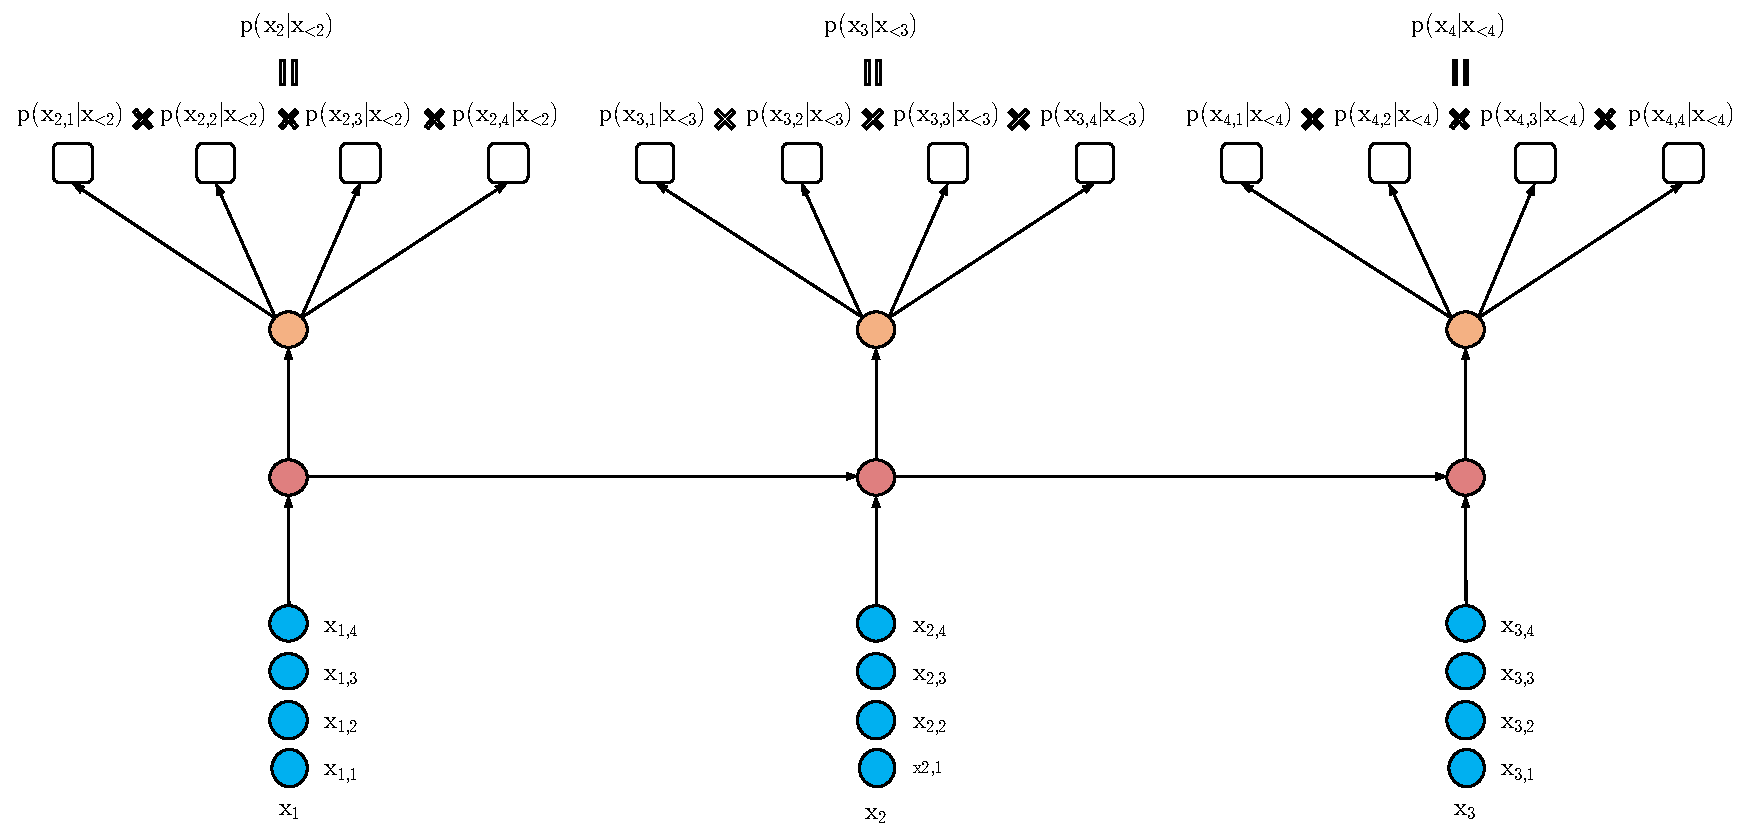
\includegraphics[width=0.85\linewidth]{fig/RNN-L4.pdf}
	\end{figure}
	\vspace{-1em}
	\begin{align*}
	\log p(\rvx) 
	= \sum_{\tau=1}^{T} \log p(\rvs_{\tau} \mid \rvs_{<\tau})
	\approx \sum_{\tau=1}^{T} \sum_{i=1}^{L} \log p(s_{\tau,i} \mid \rvs_{<\tau})
	\end{align*}
	\vspace{-1em}
  \end{block}

  \begin{block}{Basic framework - Stochastic RNN (SRNN) via VAE}
	\begin{figure}
	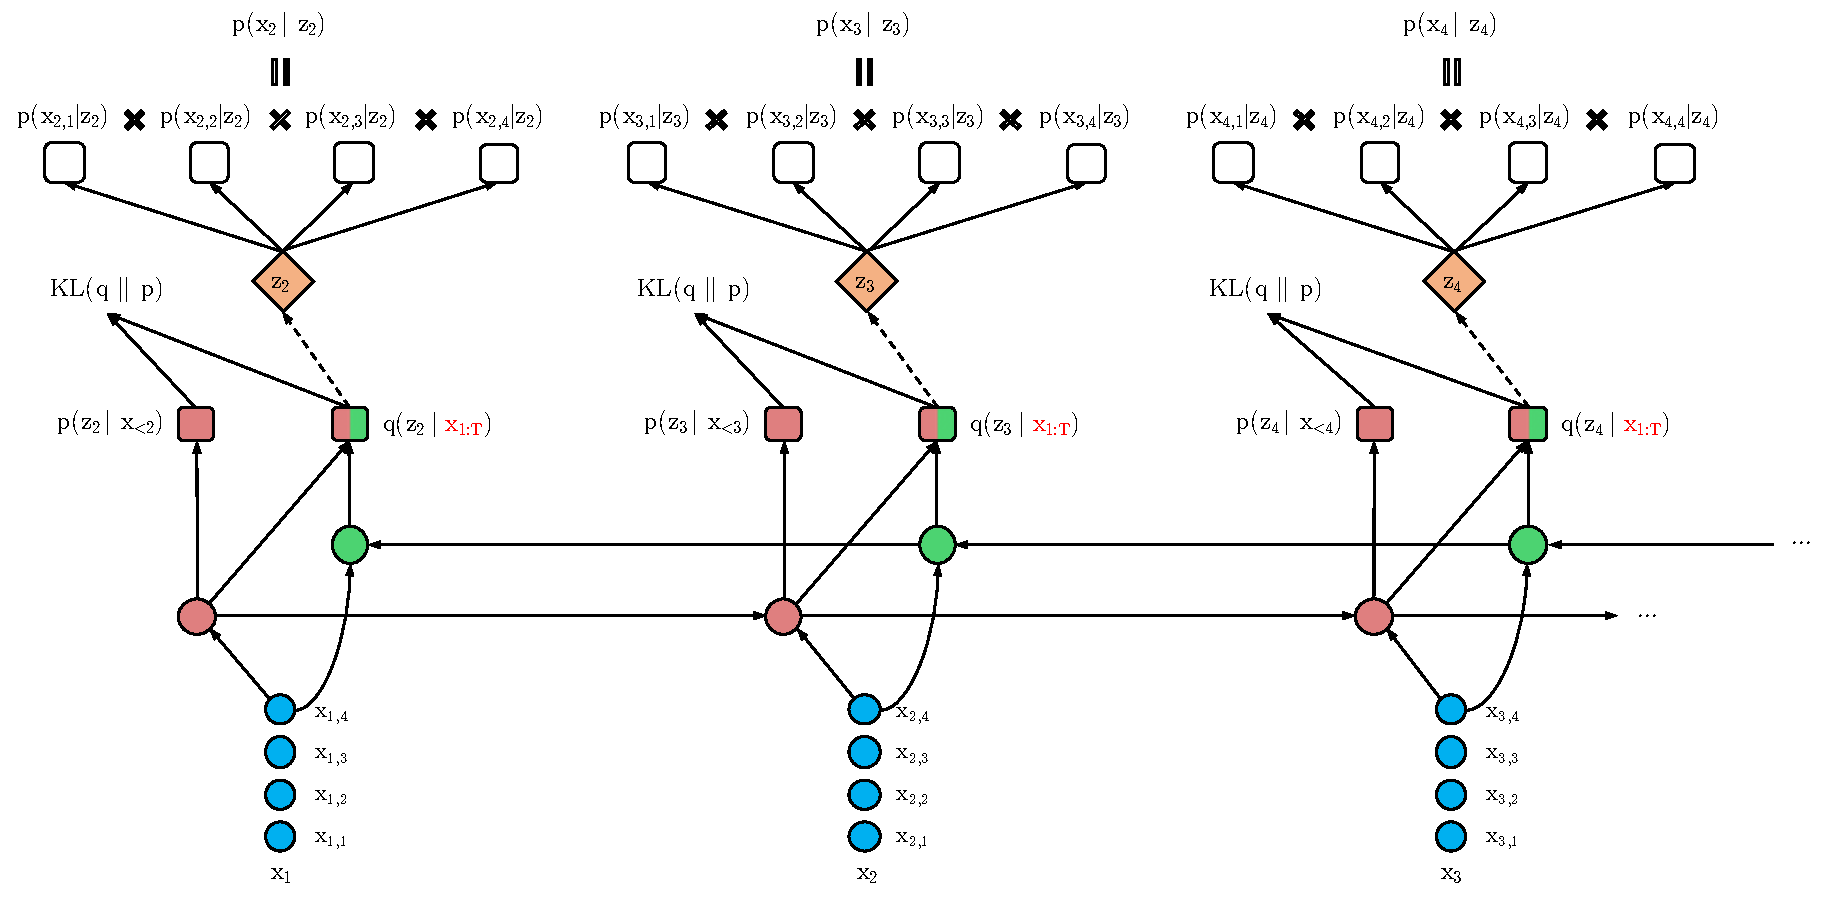
\includegraphics[width=0.85\linewidth]{fig/SRNN-L4-ELBO.pdf} % {fig/SRNN-L4-prior.pdf}
	\end{figure}
	\vspace{-1em}
	\begin{align*}
	\log p(\rvx) 
	&= \sum_{\tau=1}^{T} \log p(\rvs_{\tau} \mid \rvs_{<\tau}) 
	= \sum_{\tau=1}^{T} \log \int p(\rvs_{\tau}, \rvz_\tau \mid \rvs_{<\tau}) d\rvz_\tau && \text{(add $\rvz_\tau$ for each $\rvs_\tau$)} \\
	&= \sum_{\tau=1}^{T} \log \int p(\rvs_{\tau} \mid \rvz_\tau , \rvs_{<\tau}) p(\rvz_\tau \mid \rvs_{<\tau}) d\rvz_\tau && \text{(product rule)} \\
	&\approx \sum_{\tau=1}^{T} \log \int \sbr{ \prod_{i=1}^{L} p(s_{\tau,i} \mid \rvz_\tau , \rvs_{<\tau}) } p(\rvz_\tau \mid \rvs_{<\tau}) d\rvz_\tau && \text{(factorized)}
	\end{align*}
\end{block}
\end{column}

\separatorcolumn

\begin{column}{\colwidth}

%  \begin{block}{Optimization of Stochastic RNN}
%	\begin{figure}
%	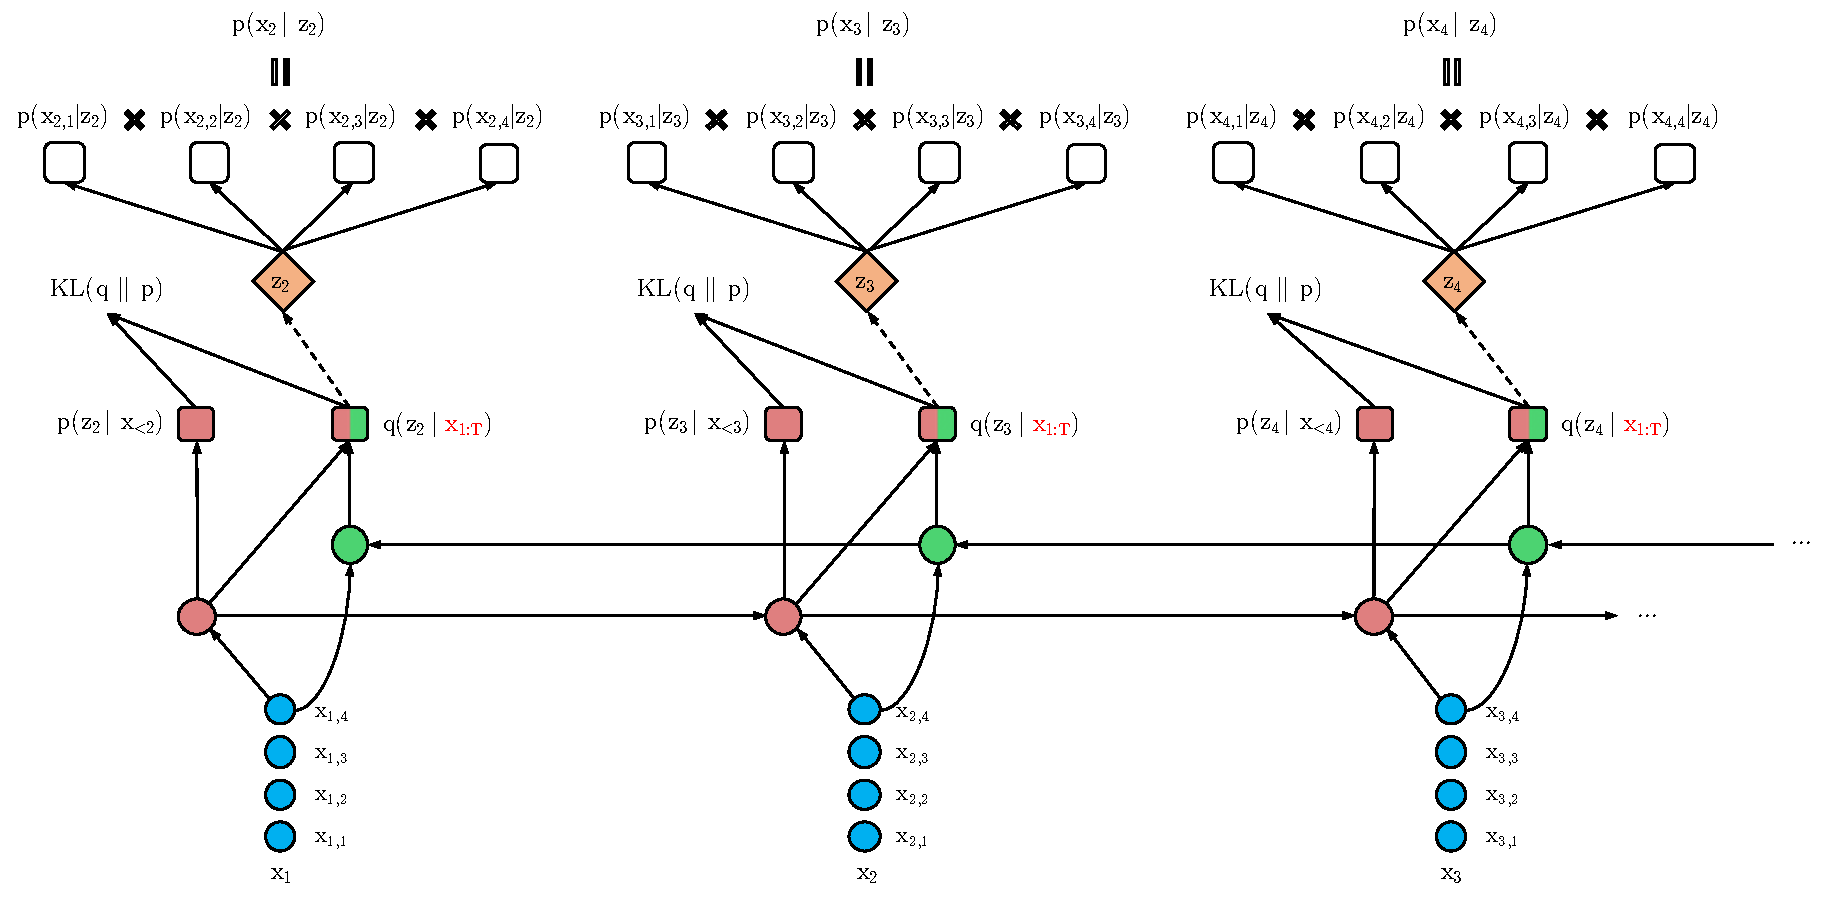
\includegraphics[width=0.9\linewidth]{fig/SRNN-L4-ELBO.pdf}
%	\end{figure}
%  \end{block}

\begin{block}{Implicit Unfairness in Capacity}
 	\textbf{RNN}: \textbf{fully factorized} prediction distribution
 	\[ 
 		p^\text{RNN}(s_{\tau} \mid \rvs_{<\tau}) \approx \prod_{i=1}^{L} p(s_{\tau,i} \mid \rvs_{<\tau})
 	\]
 	\textbf{SRNN}: \textbf{NOT} fully factorized anymore due to the integration
 	\[
 		p^\text{SRNN}(s_{\tau} \mid s_{<\tau}) \approx \int  \prod_{i=1}^{L} p(s_{\tau,i} \mid \rvs_{<\tau}, \rvz_\tau) p(\rvz_\tau \mid \rvs_{< \tau}) d \rvz_\tau
 	\]
 	
 	\textbf{In summary},
 	\begin{itemize}
 	\item SRNN is able to model the correlation within each step $\rvs_\tau$, i.e. $\set{s_{\tau,i}}_{i=1}^{L}$
 	\item RNN does not have the capacity due to the fully factorized design
 	\end{itemize}
\end{block}

\begin{block}{How does SRNN model the intra-step correlation?}
	Examine the ELBO for a prediction step $\tau$:
	\begin{equation}\label{eqn:elbo}
		\mc{L}^\text{SRNN}_\tau = \E_{\rvz_\tau \sim q(\rvz_{\tau} \mid \rvx)} \sbr{ \sum_{i=1}^{L} \log p(s_{\tau,i} \mid \rvz_\tau, \rvs_{<\tau}) } - \text{KL}\rbr{q(\rvz_{\tau} \mid \rvx) \| p(\rvz_{\tau} \mid \rvs_{<\tau})}
	\end{equation}
	\textbf{Observation}: $\rvz_{\tau}$ conditions on $\rvs_\tau$ ($\rvx$ includes $\rvs_\tau$) $\implies$ SRNN can \textbf{leak ``\cyan{partial information}''} of $\rvs_{\tau}$ through $\rvz_{\tau}$
	\begin{itemize}
		\item \textbf{Recon. term}: the cost of predicting the rest of the information \textbf{given the ``\cyan{partial information}''}
		\item \textbf{KL term}: the cost of \textbf{obtaining the ``\cyan{partial information}''}
	\end{itemize} 
\end{block}

\begin{alertblock}{A concrete example}
 	(I) Assume $\rvz_{\tau} = s_{\tau, L} \in \R$, i.e., leak the last element of $\rvs_{\tau}$ as the partial information. Formally,
 	\[ q(\rvz_{\tau} \mid \rvx) = \delta_{\rvz_{\tau} = s_{\tau, L}} = 
 	\begin{cases}
 	\infty, & \text{if $\rvz_{\tau} = s_{\tau, L}$} \\
 	0, &\text{if $\rvz_{\tau} \neq s_{\tau, L}$} \\
 	\end{cases} 
 	\]
 	
 	(II) Plug this term into ELBO equation \eqref{eqn:elbo}:
 	\begin{align*}
 	\mc{L}^\text{SRNN}_\tau
 	&= \cancel{ \gray{ \sbr[\bigg]{ \log p(s_{\tau,L} \mid s_{\tau,L}, \rvs_{<\tau}) - \log q(s_{\tau,L} \mid \rvx) } } } && \text{$\implies$ cancel out} \\
 	&+ \sbr[\bigg]{ 
 		\underbrace{\vphantom{\sum_{i=1}^{L-1}} \log p(s_{\tau,L} \mid \rvs_{<\tau})}_\text{Predict $s_{\tau,L}$ first} + 
 		\underbrace{\sum_{i=1}^{L-1} \log p(s_{\tau,i} \mid s_{\tau,L}, \rvs_{<\tau}) }_\text{Predict others conditioned on $s_{\tau,L}$}}
 	\end{align*}
 	
 	(III) Compare SRNN with RNN:
 	\begin{align*}
 	\mc{L}^\text{SRNN}_\tau
 	&= \log p(s_{\tau,L} \mid \rvs_{<\tau}) + \sum_{i=1}^{L-1} \log p(s_{\tau,i} \mid \magenta{s_{\tau,L}}, \rvs_{<\tau}) \\
 	\mc{L}^\text{RNN}_\tau
 	%  &= \sum_{i=1}^{L} \log p(s_{\tau,i} \mid \rvs_{<\tau}) \\ 
 	&= \log p(s_{\tau,L} \mid \rvs_{<\tau}) + \sum_{i=1}^{L-1} \log p(s_{\tau,i} \mid \rvs_{<\tau})
 	\end{align*}
 	\begin{itemize}
 		\item Addition intra-step dependency \magenta{\bf shown in SRNN} that is \cyan{\bf absent in RNN}
 	\end{itemize}
\end{alertblock}

\textbf{Question}: what if we allow RNN to model intra-step dependency?

\end{column}

\separatorcolumn

\begin{column}{\colwidth}

\begin{block}{Simulate information leak with RNN}
	(I) Consider a more general case:
	\begin{itemize}
	\item Leak a subset $\rvc_\tau \subset \rvs_\tau$ of $\rvs_\tau$
	\item Predict the rest $\rvs_\tau \backslash \rvc_\tau$ given $\rvc_\tau$
	\end{itemize}
	  
	(II) Simulate the case in RNN with the following objective function:
	\begin{align*}
		\log p(\rvs_{\tau} \mid \rvs_{<\tau}) \approx \log p(\rvc_{\tau} \mid \rvs_{<\tau}) + \log p(\rvs_{\tau} \backslash \rvc_{\tau} \mid \rvs_{<\tau}, \rvc_{\tau})
	\end{align*}
	
	(III) Two strategies to construct the subset $\rvc_{\tau}$:
	\begin{itemize}
		\item Interleave, every $U$ elements: $\rvc_{\tau} = \seq{s_{\tau,1}, s_{\tau,U+1}, s_{\tau,2U+1}, \cdots }$
		\item Randomly choose $V$ distinct elements : $\rvc_{\tau} = \text{random}(\rvs_{\tau}, V)$
	\end{itemize}

	\begin{table}[!h]
		\small
		\centering
		\begin{tabular}{l|c c c}
			\toprule
			\bf Models               & \bf TIMIT  & \bf VCTK  & \bf Blizzard \\
			\midrule
			RNN                       & 32,745     & 0.786     & 7,610  \\
			SRNN                      & 69,296       & \bf 2.383 & 15,258 \\
			\midrule
			$\delta$-RNN ($U = 2$)   & 70,900     & 2.027     & \bf 15,306 \\
			$\delta$-RNN ($U = 3$)   & \bf 72,067 & 2.262     & 15,284 \\
			\midrule
			$\delta$-RNN ($V = 50$)  & 66,122     & 2.199     & 14,389 \\
			$\delta$-RNN ($V = 75$)  & 66,453     & 2.120     & 14,585 \\
			\bottomrule
		\end{tabular}
		\caption{Performance comparison between $\delta$-RNN and SRNN. Note that a smaller $U$ corresponds to leaking more elements. In these experiments, $L=200$}
		\vspace{-1.5em}
		\label{tab:inter_step_correlation}
	\end{table}
\end{block}

\begin{block}{Modeling Intra-step Correlation with an Auto-Regressive Structure}
	Introduce the auto-regressive structure in both RNN \& SRNN:
	\begin{align}
	\label{eqn:ar_rnn_out_dist}
	p_\theta^\text{RNN-hier}(s_t \mid \rvs_{<t})
	&= \prod_{i=1}^{L} p_{\theta}(s_{t,i} \mid \rvs_{<t}, x_{t,<i}), \\
	\label{eqn:ar_srnn_out_dist}
	p_\theta^\text{SRNN-hier}(s_t \mid \rvz_{\le t}, \rvs_{<t})
	&= \prod_{i=1}^{L} p_{\theta}(s_{t,i} \mid \rvz_{\le t}, \rvs_{<t}, x_{t,<i}).
	\end{align}
	\begin{table}[!t]
		\centering
		\small
		\begin{tabular}{l|c c c | c c }
			\toprule
			\bf Models          & \bf TIMIT & \bf VCTK  & \bf Blizzard  & \bf Muse  & \bf Nottingham \\
			\midrule
			VRNN~\cite{chung2015recurrent}      & 28,982      & -          & 9,392      &  -         &  -      \\
			SRNN~\cite{fraccaro2016sequential}      & 60,550      & -          & 11,991     &  -6.28     &  -2.94     \\\
			Z-Forcing~\cite{goyal2017z}  & 70,469 & -          & 15,430     &  -         &  -       \\
			\midrule
			RNN               & 32,745      & 0.786      & 7,610     & -6.991     & -3.400     \\
			\midrule\midrule
			RNN-hier            & \textbf{109,641}     & \textbf{3.1822}     & \textbf{21,950}     & \textbf{-5.161} & \textbf{-2.028} \\
			SRNN-hier           & 107,912     & 3.1423     & 21,845     & -5.483     & -2.065    \\
			\bottomrule
		\end{tabular}
		\caption{Performance comparison on a diverse set of datasets. - suggests the model is not application on the dataset. }
		\label{tab:non_factorized}
		\vspace{-1.5em}
	\end{table}
	\vspace{-1.0em}
\end{block}

\begin{block}{Conclusion}
	(1) Latent variables provides a mechanism to leverage the intra-step correlation
	
	(2) However, its capacity is clearly weaker compared to a simple auto-regressive structure
%  	From our empirical observation, the main effect of latent variables is only to provide a mechanism to leverage the intra-step correlation, which is however, not as powerful as employing the straightforward auto-regressive decomposition.
%  	It remains unclear what leads to the significant gap between the theoretical potential of latent variables and their practical effectiveness, which we believe deserves more research attention.
%  	\vspace{-1.0em}
\end{block}

\begin{block}{References}
	\vspace{-0.2em}
    \nocite{*}
	\setbeamertemplate{bibliography entry article}{}
	\setbeamertemplate{bibliography entry title}{}
	\setbeamertemplate{bibliography entry location}{}
	\setbeamertemplate{bibliography entry note}{}
    \footnotesize{\bibliographystyle{plain}\bibliography{poster}}
\end{block}

\end{column}

\separatorcolumn
\end{columns}
\end{frame}

\end{document}
